\part{Traitements, calculs}
\label{part:traite}

\section{L'interpréteur de commandes : \texttt{adc}}

  Le système de traitement d'AIDA est construit autour d'un
langage de commande, qui permet d'exécuter des fonctions
de traitement sur des données choisies.

\medbreak
\textbf{\textit{Note : adc est le résultat de la réécriture en langage Python
de l'interpréteur de commande initial (écrit en langage C) : fvb}}

\subsection{Le langage}

Une ligne de commande doit avoir la forme suivante :

\fbox{ \texttt {opérateur ( argument [, autre\_argument] )} }

\medbreak
Une ligne de commentaire commençe par \texttt{\#} :

\fbox{ \texttt{\# commentaire }} \\

\bigbreak
On appelle \texttt{opérateur} une fonction de calcul qui a deux
particularités :
\begin{itemize}
  \item d'une part, cette fonction travaille sur l'ensemble de la série
        temporelle de mesure,
  \item d'autre part, elle est décrite de façon plus complète qu'une fonction
        d'un langage de programmation classique, ce qui permet au système de
        mieux vérifier les arguments en entrée, et de mieux renseigner les
        attributs des résultats (en particulier pour leur unité).
\end{itemize}

\medbreak
L'ensemble des opérateurs disponibles est documenté dans le catalogue : \\
\texttt{\$AIDA\_HOME/doc/CATALOG\_OPER.pdf}.

\medbreak
Les arguments peuvent être :
\begin {itemize}
  \item le nom d'une série de mesure (nom du ``vecteur'', pas du fichier)
  \item un nombre
  \item une constante symbolique de la liste ci-dessous
        (voir : \ref{sec:Cste}, page \pageref{sec:Cste}).
  \item une référence à un attribut de l'acquisition. \\
        La syntaxe est alors : \\
        \texttt{\$Acq.<nom\_rubrique>.<nom\_attribut>}
        (voir : \ref{sec:Acq}, page \pageref{sec:Acq}).
  \item une référence à un attribut d'un argument précédent. \\
        La syntaxe est alors : \\
        \texttt{\$Arg\textit{xx}.nom\_attribut}
        (voir : \ref{sec:Arg}, page \pageref{sec:Arg}).
  \item une valeur de paramètre qui évolue dans le temps. \\
        La syntaxe est alors : \\
        \texttt{\$Chrono.PARAM}
        (voir : \ref{sec:Chrono}, page \pageref{sec:Chrono}).
  \item une formule utilisant un nombre, une constante ou un attribut. \\
        Les opérations connues sont : +-*/
  \item un paramètre optionnel de l'opérateur
        (voir : \ref{sec:param_opt_oper}, page \pageref{sec:param_opt_oper}).
  \item un paramètre optionnel de \texttt{adc}.
        (voir : \ref{sec:param_opt_adc}, page \pageref{sec:param_opt_adc}).
\end {itemize}

\subsubsection{Les constantes symboliques}
  Elles sont définies dans le fichier : \\
\-\hspace{1cm} \texttt{\$AIDA\_HOME/src/python3/AIDA\_lib/Constantes.py}. \\
Les \textit{constantes simples} sont les suivantes :

\label{sec:Cste}
\begin{tabular}{l|l|l}
 nom          & type       & valeur \\
\hline
 ieeefloat64\_max & double  & 1.7976931348623157e+308 \\
 ieeefloat32\_max & float  & 3.40282347e+38 \\
 int32\_max    & int\_32  & 2147483647 \\
 int16\_max    & int\_16  & 32767 \\
 pi           & double  & 3.14159265358979323846 \\
 DegRad       & double  & 3.14159265358979323846 / 180.0 \\
 RadDeg       & double  & 180.0 / 3.14159265358979323846 \\
 KtMs         & double  & 1852.0 / 3600.0 \\
 FtmMs        & double  & 0.3048 / 60.0 \\
 FtM          & double  & 0.3048 \\
 g            & double  & 9.806650 \\
 T0           & double  & 273.15 \\
 sigma        & double  & 5.67051e-8 \\
 sigma\_LOA    & double  & 5.6698e-8 \\
 R            & double  & 8.314510 \\
 Ra           & double  & 8.314510 / 0.028964 \\
 Rv           & double  & 461.51 \\
 cpa          & double  & 1004.685 \\
 cva          & double  & 717.64 \\
\end{tabular}

\medbreak
  Se référer directement au fichier des constantes pour les valeurs des
\textit{constantes plus compliquées} :
\begin{verbatim}
- SA_PMS_OAP230Y
- SA_PMS_OAP200X_INSU
- SA_PMS_OAP200X_LaMP
- FSSP300_std_mid_diam
- SPP200_std_mid_diam
- PCASP_std_mid_diam
- GRIMM1_109_std_mid_diam
\end{verbatim}

\subsubsection{Les attributs de l'acquisition \$Acq}
\label{sec:Acq}
  La syntaxe générale est : \\
\texttt{\$Acq.<nom\_rubrique>.<nom\_attribut>}

\medbreak
  Les dates sont des quantités qui peuvent être exprimées de plusieurs manières,
une syntaxe spécifique a donc été mise en place. La forme générale est : \\
\texttt{\$Acq.\$nom\_de\_la\_date.quantité}.

\bigbreak
Actuellement, la seule syntaxe utilisable est : \\
\fbox{ \texttt{\$Acq.\$date.DOY} } \\
qui donne la date d'acquisition (champ \texttt{date} de la rubrique
\texttt{[IDENTIFICATION]} du fichier .inf), exprimée sous la forme d'un numéro
du jour dans l'année.


\subsubsection{Les attributs des arguments \$Arg}
\label{sec:Arg}
Les noms des attributs des arguments correspondent
généralement aux noms des champs de l'en-tête des
fichiers vecteurs, à quelques exceptions près, soit
pour des raisons historiques (sample, array\_dim), soit
pour désigner une information qui n'existe pas
dans l'en-tête (NbVal).

\begin{tabular}{r l}
 \textbf{Nom}          & \textbf{Signification}  \\
\hline
 nom & le nom du vecteur (chaîne de caractère)\\
 array\_dim & la dimension de chaque échantillon (nombre)\\
 array\_shape & dimensions (au sens shape) des données (chaîne de caractère)\\
 sample & la fréquence d'échantillonnage (nombre)\\
 NbVal & le nombre d'échantillons (nombre)\\
 unit & l'unité (chaîne de caractère) \\
 time\_bnds & bornes temps (chaîne de caractère)\\
 misval & la valeur manquante (même type que le vecteur) \\
 famille & la famille du paramètre (chaîne de caractère ) \\
 name & le nom long (chaîne de caractère ) \\
 english\_name & le nom long en anglais (chaîne de caractère ) \\
\end{tabular}

\subsubsection{Les attributs \$Chrono}
\label{sec:Chrono}
Les attributs de type \$Chrono.PARAM permettent de gérer des paramètres de
traitement qui évoluent avec le temps. La valeur de PARAM est lue dans un
fichier de configuration associé à la plateforme dans lequel sont décrites
les valeurs que prend PARAM en fonction de la date. Ce fichier est décrit
dans le document de référence volume 1 : \url{refman.pdf}.

\subsubsection{Les paramètres optionnels de l'opérateur}
\label{sec:param_opt_oper}
Certains opérateurs peuvent accepter des arguments optionnels.
Ceux-ci sont présentés dans la documentation de l'opérateur sous la rubrique :
\textbf {Entrées optionnelles}.

La forme générale pour fournir un argument optionnel dans la ligne de commande
est : \fbox{ \texttt {<argument>=<valeur>} }
\medbreak

La forme de la valeur de l'argument optionnel dépend du type de l'argument
définit dans la documentation de l'opérateur:

\begin{itemize}
  \item[•] \texttt{NUM}    : l'argument attendu est un numérique (entier,
                             flottant, etc). \\
                             Ex : \texttt{value=12}

  \item[•] \texttt{list()} : l'argument attendu est une liste python. \\
                             Ex : \texttt{value=[0, 100]}

  \item[•] \texttt{dict()} : l'argument attendu est un dictionnaire python. \\
                             Ex : \texttt{value=\{"min"=0, "max"=100]\}}

  \item[•] \texttt{bool()} : l'argument attendu est un booléen python
                             (True, False). \\
                             Ex : \texttt{value=True}

  \item[•] \texttt{str()}  : l'argument attendu est une chaîne python \\
                             Ex : \texttt{value="radian"}

\end{itemize}

\subsubsection{Les paramètres optionnels de adc}
\label{sec:param_opt_adc}

Ces paramètres sont traités directement par \texttt{adc} (on peut donner
autant de paramètres de type que nécessaire).

Ils permettent de remplacer la valeur d'un champ du header des vecteurs de
sortie par une valeur définie par l'utilisateur. \\
Ils permettent également de créer un champ dans le header des vecteurs de
sortie.
\medbreak

La forme générale pour fournir un argument optionnel de \texttt{adc} dans la
ligne de commande est : \fbox{ \texttt{HDR\_xxx=[..., ...]} }
\medbreak
  où : \texttt{xxx} est le nom d'un champ du header du vecteur de sortie
  existant ou \textbf{à créer} (Ex : \texttt{HDR\_english\_name},
  \texttt{HDR\_SPECIAL\_comment}).
\medbreak

La partie entre crochets (\texttt{[]}) doit contenir autant de valeurs
de remplacement que de vecteurs de sortie de l'opérateur, séparées par des
virgules (\texttt{','}). \\
Si pour un vecteur de sortie \texttt{adc} ne doit par modifier la valeur
positionnée par l'opérateur, sa valeur doit être : \texttt{None}. \\
\medbreak

Exemple : pour un opérateur qui génère 3 vecteurs de sortie, si l'appel de
l'opérateur contient : \\
\textbf{\texttt{ HDR\_english\_name=['new name for param x', None, 'new name for param z']}} \\
alors : \\
\begin{itemize}
  \item[•] le vecteur de sortie n°1 contiendra :
	       \texttt{english\_name = new name for param x}
  \item[•] le vecteur de sortie n°2 contiendra :
           \texttt{english\_name = <l'english\_name calculé par l'opérateur>}
  \item[•] le vecteur de sortie n°3 contiendra :
           \texttt{english\_name = new name for param z}
\end{itemize}
\medbreak

Exemple : pour un opérateur qui génère 1 vecteur de sortie, si l'appel de
l'opérateur contient : \\
\textbf{\texttt{ HDR\_SPECIAL\_comment=['commentaire'] }} \\
alors : \\
\begin{itemize}
  \item[•] le vecteur de sortie contiendra : \texttt{SPECIAL\_comment = commentaire}
\end{itemize}
\medbreak


\subsection{Exemples}

\textbf{\textit{Note : l'écriture de fichier de commande pour adc (.fil) est
grandement facilitée par l'utilisation de l'interface graphique \texttt{edifil}
(voir \nameref{sec:edifile})}}

\subsubsection{Exemple d'appel d'un opérateur}

La ligne de commande pour calculer la somme de deux vecteurs (qui doivent
être synchrones, bien sûr) est : \\
\texttt{Plus (<nom\_premier\_vect>, <nom\_second\_vect>, <nom\_résultat>)}

\subsubsection{Exemple de fichier de commandes de traitement (.fil)}
\newgeometry{margin=1cm}
\begin{landscape}
\thispagestyle{mylandscape} %Call our predefined page type
  \begin{lstlisting}
    # Traitement des donnees pluvio
    # - Calculs de précipitation de la station meteopole-flux
    
    # Quantité de précipitation sur 1 mn
    # (pluvio de reference de la DSO reférencé dans le fichier chrono)
    Ech_tps_impos ($Chrono.CHOIX_PLUVIO, $Chrono.REFTIME_PLUVIO, 60., rft_time_REG_%60, $Arg4.NbVal, prp_rr_min_c2_Eti_%60) 
    
    # On effectue un remplissage avec des valeurs nulles pour le flag = 2
    Remplace_selon_flag (prp_rr_min_c2_Eti_%60, ctl_flag_invalid_pluvio_%60, 1.9, 2.1, 0, prp_rr_min_c2_remplac_%60)
    
    # On interpole pour eviter la valeur manquante sur la derniere minute
    Correc_hors_bornes (prp_rr_min_c2_remplac_%60, 0.,100.,1,$Arg1.misval, prp_rr_min_c2_Chb_%60)
    Poly_1_flt (prp_rr_min_c2_Chb_%60,0.,1.0, "mm" , "", "", prp_rr_min_c2_mm_%60) 
    
    # Cumul des quantités de precipitation sur 1 heure
    Som(prp_rr_min_c2_mm_%60,60,0, prp_rr_cumul_%60_%3600)
    
    # Calcul de la série quotidienne de cumul de RR
    Cumul (prp_rr_min_c2_Chb_%60, prp_rr_auto_cumule_%60)
  \end{lstlisting}
\end{landscape}
\restoregeometry


\subsection{Lancement}
\texttt{adc} peut être lancé sous \texttt{aito} par l'intermédiaire de l'outil
\texttt{edifil} (bouton \texttt{edifil})
ou en ligne de commande dans un terminal :

\fbox{ \texttt{adc  [options] acqids [Fichier\_de\_commandes\_de\_traitement]} }

\medbreak
avec : \\
\begin{itemize}
  \item[•] \texttt{acqids} : un identificateur d'acquisition unique
    \textbf{ou} une séquence d'identificateurs. Dans ce dernier cas, la
    forme est : \texttt{<premier\_acqid>-<dernier\_acqid>}. \\
    Ex :
    \begin{itemize}
      \item as200015 : le traiement sera appliqué à la seule acquisition as200015.
      \item as200015-as200019 : le traiement sera appliqué à toutes les
            acquisitions comprises entre [as200015, as200019].
    \end{itemize}

  \item[•] \texttt{[Fichier\_de\_commandes\_de\_traitement]} : fichier
    contenant les commandes adc à appliquer à \texttt{acqids}.
    Usuellement, l'extension du nom de ce type de fichier est
    \texttt{\textbf{.fil}}. \\
    Si cet argument optionnel n'est pas donné, les commandes sont lues sur
    l'entrée standard.

  \item[•] Sans option : le résultat est écrit sur disque si
    le vecteur n'existe pas.

  \item[•] Les options possibles sont les suivantes :
    \begin{description}
      \item -h : affiche un court texte d'aide.

      \item -v : affiche des informations de version.

      \item -V : mode \textit{Verbose}. Augmente le niveau des traces écran.

      \item -S : mode \textit{stop on error}.  Arrêt de adc à la première
                 erreur rencontrée. \textit{Défaut} : False

      \item -M <mail-list> : mode \textit{mail-to}. Le fichier de
                 configuration \\
                 \texttt{\$AIDA\_HOME/profils/\$AIDA\_PROFIL/AIDA\_mail.cfg}
                 doit exister (voir : \ref{ex:mail}, page \pageref{ex:mail}).
                 Les adresses sont séparées par des virgules (,) sans espaces.

      \item -f : mode \textit{versionning}. Les résultats sont toujours écrits
                 sur disque/base, en créant éventuellement une version de
                 sauvegarde (\texttt{<paramètre>.vx.vbn}) d'un paramètre de
                 même nom déjà existant.

      \item -F : mode \textit{force}. Les résultats sont toujours écrits sur
                 disque/base, en remplaçant éventuellement un paramètre de
                 même nom déjà existant.

      \item -N<i> : mode \textit{développement}. Les résultats sont toujours
                    écrits sur disque, une version n<i> est créée
                    (\texttt{<paramètre>.n<i>.vbn}).

      \item -C : invalide le contrôle sur les familles.
                 Cette option permet de retraiter les anciennes acquisitions
                 comme le faisait fvb (qui ne faisait pas ce contrôle)

      \item -T : mode \textit{test et validation}. Avant d'écraser un vecteur
                 xxx.vbn, généré par fvb, adc le renomme xxx.FVB.vbn. Ce
                 vecteur pourra, par la suite, être utilisé par l'outillage de
                 validation du répertoire :
                 \path{src/python3/packages/AIDAcalc/validation}.
    \end{description}
\end{itemize}


\subsubsection{Exemple de fichier de configuration des mails automatiques}
 \label{ex:mail}
 \begin{lstlisting}
  # configuration pour les mails automatiques
  [AIDAcalc]
  smtp      = smtp.xxx.yyy
  from_addr = aaa.bbb@domaine
 \end{lstlisting}


\section{IHM graphique de adc : \texttt{edifil}}
\label{sec:edifile}
L'interface graphique \texttt{edifil} permet d'écrire des fichiers de
commandes pour l'interpréteur de commande \texttt{adc} (fichiers \texttt{.fil}
décrits ci-dessus). \texttt{edifil} permet également de tester ou exécuter
les fichiers \texttt{.fil} sur un \texttt{acqid}.

\subsection{Lancement}
\texttt{edifil} peut être lancé sous \texttt{aito} (bouton \texttt{edifil})
ou en ligne de commande dans un terminal :

\fbox{ \texttt{edifil.py [\textit{options}] [\textit{file ...}]} }

\medskip

avec :

\begin{itemize}
\item[•] \textit{options} :
    \begin{itemize}
      \item[] \texttt{-h/{}-{}-help}                    : affiche l'aide.
    \end{itemize}

\item[•] \textit{file ...} : argument facultatif. Un ou plusieurs fichiers de
                             commandes pour adc (.fil)
\end{itemize}

\medskip


\subsection{Présentation}
La page principale de \texttt{edifil} comporte plusieurs parties :

\begin{center}
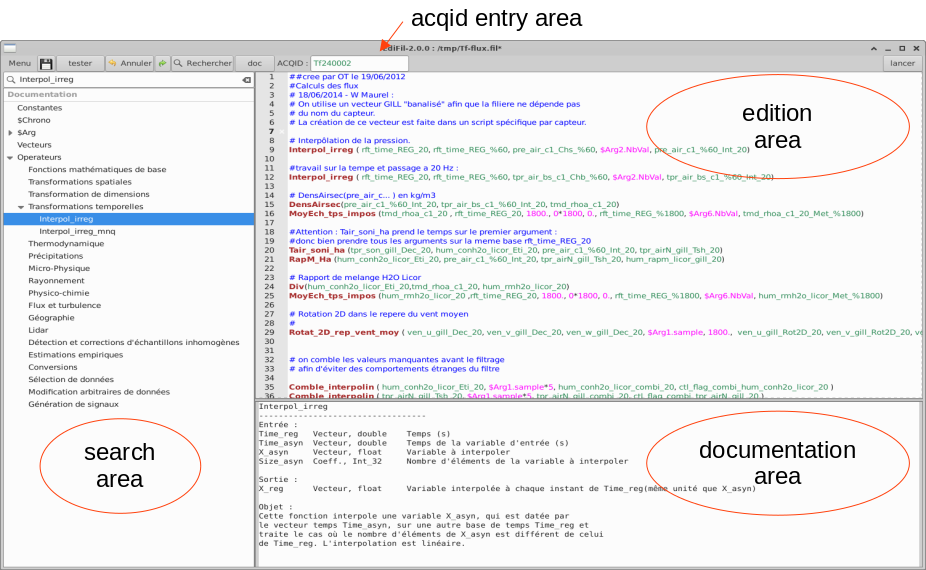
\includegraphics[width=14cm]{images/edifil.png}
\end{center}

L'aide de \texttt{edifil} est présentée sous l'entrée \textbf{Aide du Menu}.
